\subsection{Product perspective}
\subsubsection{Class diagrams}
The following pages present the UML class diagrams which represent the elements that are relevant to the domain of the application. Only the relevant parts of the system are present for the sake of clarity.
\begin{figure}[H]
    \centering
    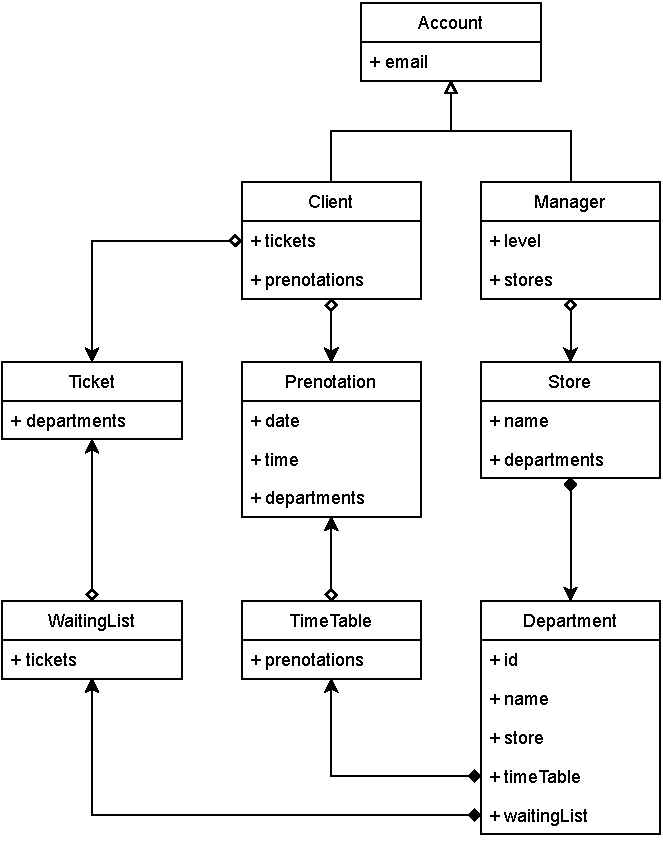
\includegraphics{Images/main-class-diag.pdf}
    \caption{\label{fig:metamodel}High level class diagram}
\end{figure}

\newpage
\subsubsection{State machine diagrams}
The following diagrams represent a high level description of the evolution of the states of the system during its processes.

\begin{figure}[H]
    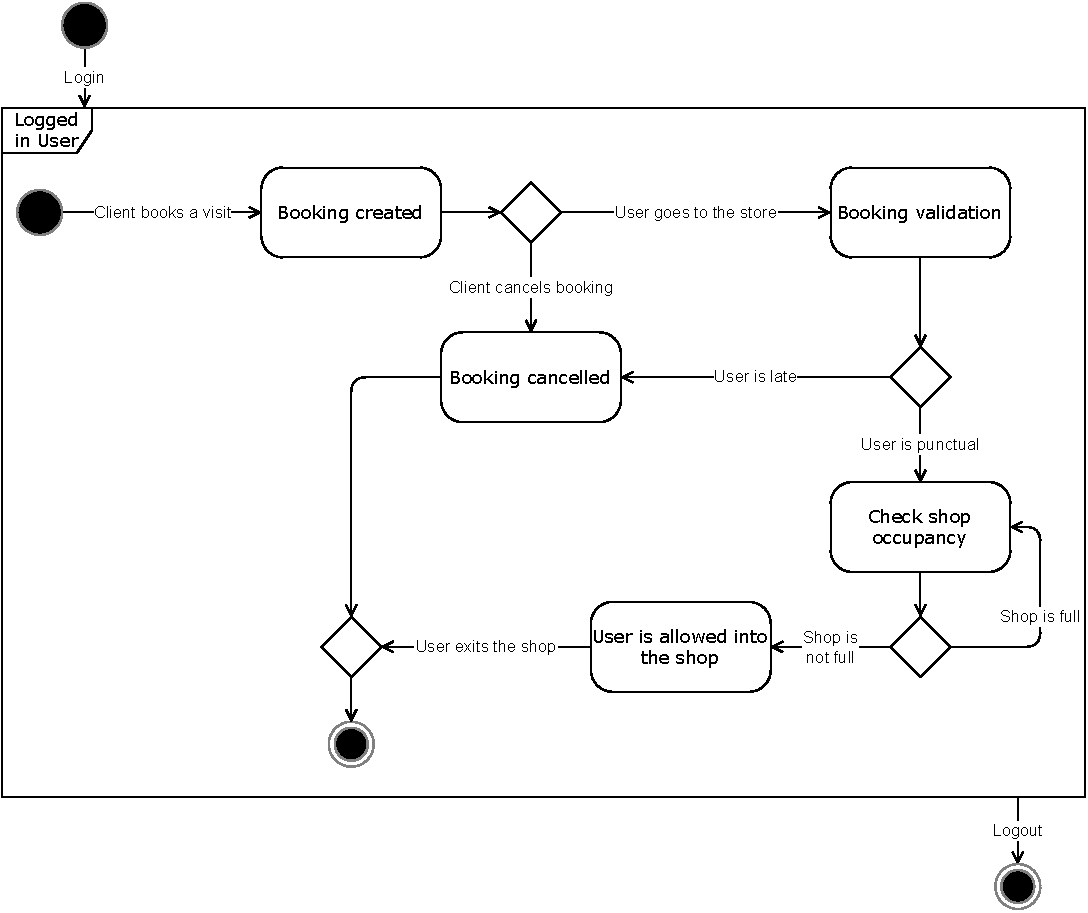
\includegraphics[width=\linewidth]{Images/state-diag-Booking.pdf}
    \caption{Statechart of the lifetime of a Booking}
    \label{fig:statechart_booking}
\end{figure}

\begin{figure}[H]
    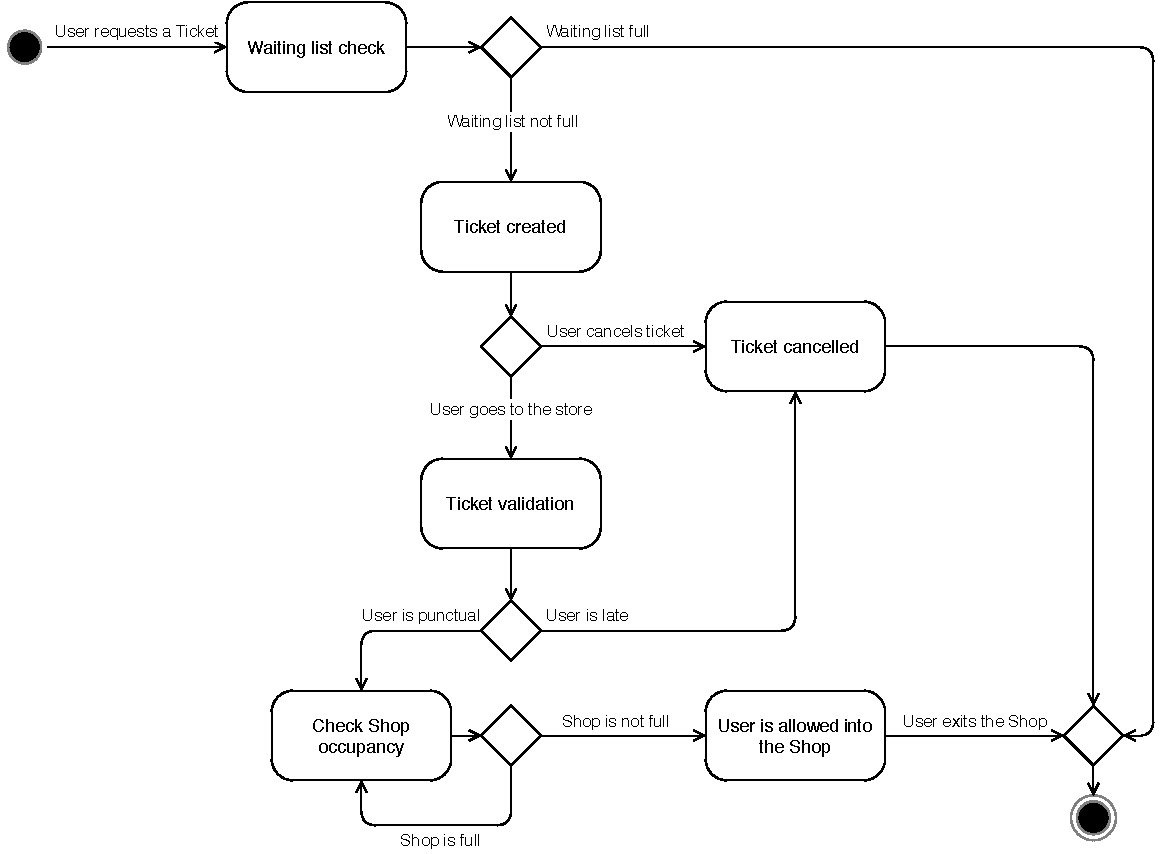
\includegraphics[width=\linewidth]{Images/state-diag_Ticket.pdf}
    \caption{Statechart of the lifetime of a Ticket}
    \label{fig:statechart_ticket}
\end{figure}

\begin{figure}[H]
    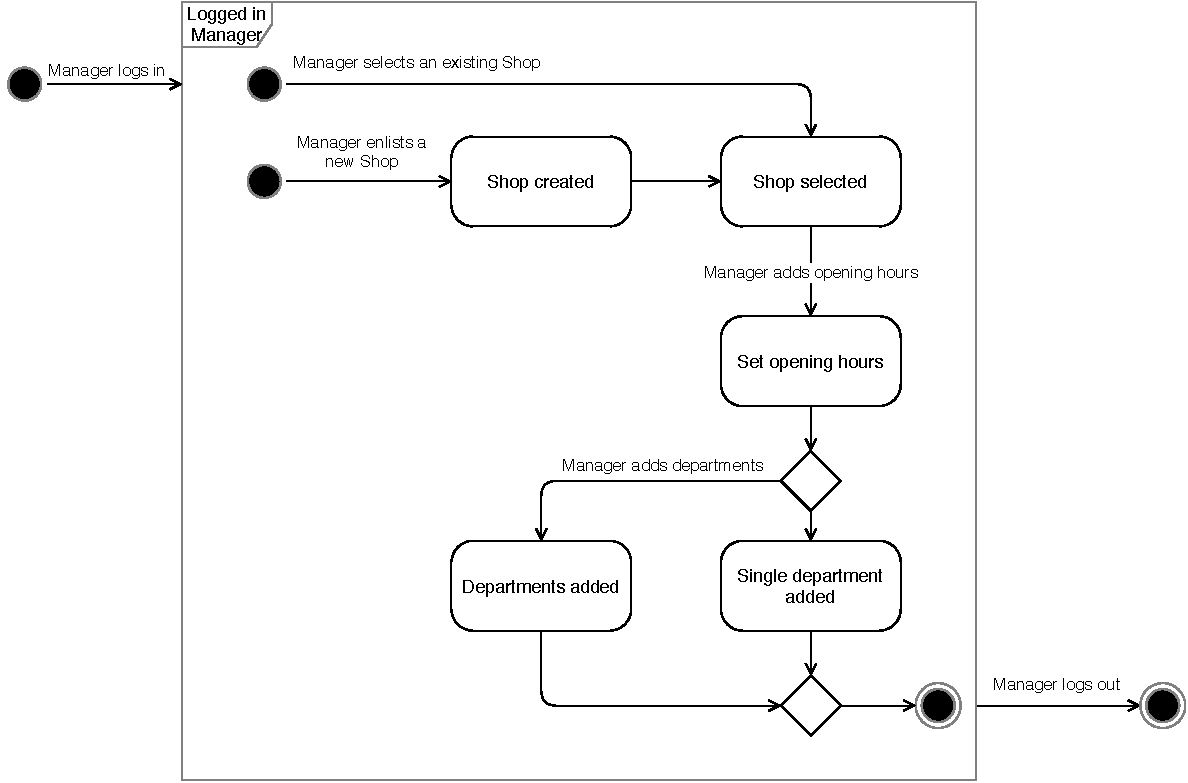
\includegraphics[width=\linewidth]{Images/state-diag_Manager.pdf}
    \caption{Statechart of the Shop creation and configuration}
    \label{fig:statechart_manager}
\end{figure}



\subsection{Product functions}
\emph{CLup} offers the Customers two ways of accessing a Third Party Shop: they can request a Ticket to for an immediate visit, or make a Booking for a future visit. The proofs of reservation (Ticket or Booking) must be validated before entering the Shop. An alternative must be guaranteed on-location for customers who cannot access the service.
The configuration of Shop is handled by the Third Party, which is able to set the opening times and the departments. When \emph{CLup} is operative, the Third Party can monitor the occupancy of the Shop, detailed into the various departments.
\\Here is an overview of \emph{CLup} functions, subdivided into three sets, related to the Customers, the Third Party clerks and the Third Party managers:

\paragraph{Basic Customer functions} These functions are available to all Customers:
\begin{itemize}
    \item \textbf{Registration and Login}\\
          Customers should be able to create a personal account for the App. By logging in with their account, Customers can access the other functions. For ease of use the app should allow users to stay logged in, this way the service can be accessed without inserting the login credentials every time.
    \item \textbf{Obtaining a Ticket}\\
          \emph{CLup} has a waiting list of the customers who are currently waiting to enter the Shop. Registered Customers can request to join the list via the App, if the queue is not full for the day they will be given a ticket. The ticket is associated with a \emph{unique} Token that can be shown to the staff. Customers are granted access to the shop by showing the token to the staff when it's their turn. Notifications can be sent to the Customers' devices to remind them when it is their turn to enter the Store.
    \item \textbf{Booking a visit}\\
          \emph{CLup} keeps a table of booked visits to the Shop. Registered Customers can book a visit for a specified time and date via the App if the time slot is not full. A successful booking is associated with a \emph{unique} Token that can be shown to the staff. Customers are granted access to the shop by showing the token to the staff in the time slot they bookid. Notifications can be sent to the Customers' devices to remind them about upcoming bookings.
    \item \textbf{Specifying item categories}\\
          When booking a visit or getting a ticket, Customers can specify categories of products they intend to buy. This data can be used to better optimize the occupancy of the departments of the Shop.
\end{itemize}

\paragraph{Third Parties base functions}
These functions should be accessible to all the employees of the Third Party, since they are required for the proper working of the system, at an operational level:
\begin{itemize}
    \item\textbf{Login}\\
          Third Parties clerks and managers shall be provided with valid credentials to login into the system.
    \item\textbf{Substitute ticket distribution}\\
          Third Parties shall be able to generate a ticket for Customers who do not have the required technologies, which allows them to join the waiting list. Booking is only allowed via the App, since it requires more detailed information;
    \item \textbf{Ticket and Booking validation}\\
          \emph{CLup} allows Third Parties to check Customers' tickets against those stored in the system. This is fundamental to deny forged tickets.
\end{itemize}
\paragraph{Third Parties administration functions}
These functions must only be accessible to the managers of the Third Party, since they control administrative aspects of the service, which handle sensible or critical data:
\begin{itemize}
    \item\textbf{Shop creation and configuration}\\
          Third Parties shall be able to enlist their store in the \emph{CLup} system, specifiying opening hours and departments with the respective capacities. This is only possible with a manager account, while the clerks should only be allowed to;
    \item\textbf{Shop occupancy checking}\\
          \emph{CLup} allows Third Parties to monitor entrances, to ensure all of the imposed restrictions are being followed. These data are also a source of useful insights in a business perspective.
\end{itemize}
\subsection{Customer characteristics}

CLup is meant to be accessible for customers of all demographics.

\subsubsection{Actors}
\begin{itemize}
    \item \textbf{Customer}: people who need to go shopping
    \item \textbf{Shop manager}: someone who owns a retail commercial activity which needs to operate at limited capacity
    \item \textbf{Staff}: people working at a Shop
\end{itemize}

\subsection{Assumptions, dependencies and constraints}
\begin{description}
    \item[D1] Each customer creates only one account
    \item[D2] The information provided by the manager is correct
    \item[D3] The maximum capacity provided by the manager is compliant to active health and safety measures
    \item[D4] Most of the customers that take a ticket or book a visit will actually visit the shop
    \item[D5] The staff will validate tickets and bookings on entry and exit
    \item[D6] Transgressors will be handled by the staff
    \item[D7] Clients will be instructed to use the application if possible
    \item[D8] Shops are added by the legitimate owner
    \item[D9] Only existing shops are added to the system
\end{description}